\chapter{椭球坐标系}

% Confocal quadrics TikZ drawing commands used only in this chapter's figure.
\newcommand{\DrawConfocalAxes}[3]{%
  \draw[axes] (0,0,0) -- (#1,0,0) node[pos=1.15, anchor=west] {$x$};
  \draw[axes] (0,0,0) -- (0,#2,0) node[pos=1.1, anchor=south] {$y$};
  \draw[axes] (0,0,0) -- (0,0,#3) node[pos=1, anchor=south] {$z$};
}

\newcommand{\DrawConfocalEllipsoid}[5]{%
  \pgfmathsetmacro{\Ax}{sqrt((#1)*(#1)+(#4))}
  \pgfmathsetmacro{\By}{sqrt((#2)*(#2)+(#4))}
  \pgfmathsetmacro{\Cz}{sqrt((#3)*(#3)+(#4))}
  \foreach \v in {-60,-30,0,30,60}{%
    \draw[#5] plot[domain=0:360, samples=60, variable=\u]
      ({\Ax*cos(\u)*cos(\v)}, {\By*sin(\u)*cos(\v)}, {\Cz*sin(\v)});}
  \foreach \u in {0,30,...,150}{%
    \draw[#5] plot[domain=-80:80, samples=60, variable=\v]
      ({\Ax*cos(\u)*cos(\v)}, {\By*sin(\u)*cos(\v)}, {\Cz*sin(\v)});}
}

\newcommand{\DrawConfocalOneSheet}[6]{%
  \pgfmathsetmacro{\A}{(#1)*(#1)+(#4)}
  \pgfmathsetmacro{\B}{(#2)*(#2)+(#4)}
  \pgfmathsetmacro{\C}{-((#3)*(#3)+(#4))}
  \pgfmathsetmacro{\sA}{sqrt(\A)}
  \pgfmathsetmacro{\sB}{sqrt(\B)}
  \pgfmathsetmacro{\sC}{sqrt(\C)}
  \def\tm{#5}
  \foreach \u in {0,40,...,320}{%
    \draw[#6] plot[domain=-\tm:\tm, samples=60, variable=\t]
      ({\sA*cosh(\t)*cos(\u)}, {\sB*cosh(\t)*sin(\u)}, {\sC*sinh(\t)});}
  \foreach \t in {-0.9,-0.45,0,0.45,0.9}{%
    \draw[#6] plot[domain=0:360, samples=60, variable=\u]
      ({\sA*cosh(\t)*cos(\u)}, {\sB*cosh(\t)*sin(\u)}, {\sC*sinh(\t)});}
}

\newcommand{\DrawConfocalTwoSheet}[7]{%
  \pgfmathsetmacro{\A}{(#1)*(#1)+(#4)}
  \pgfmathsetmacro{\B}{-((#2)*(#2)+(#4))}
  \pgfmathsetmacro{\C}{-((#3)*(#3)+(#4))}
  \pgfmathsetmacro{\sA}{sqrt(\A)}
  \pgfmathsetmacro{\sB}{sqrt(\B)}
  \pgfmathsetmacro{\sC}{sqrt(\C)}
  \def\tmin{#5}
  \def\tmax{#6}
  \foreach \u in {0,60,...,300}{%
    \draw[#7] plot[domain=\tmin:\tmax, samples=60, variable=\t]
      ({\sA*cosh(\t)}, {\sB*sinh(\t)*cos(\u)}, {\sC*sinh(\t)*sin(\u)});}
  \foreach \t in {0.4,0.7,1.0}{%
    \draw[#7] plot[domain=0:360, samples=60, variable=\u]
      ({\sA*cosh(\t)}, {\sB*sinh(\t)*cos(\u)}, {\sC*sinh(\t)*sin(\u)});}
  \foreach \u in {0,60,...,300}{%
    \draw[#7] plot[domain=\tmin:\tmax, samples=60, variable=\t]
      ({-\sA*cosh(\t)}, {\sB*sinh(\t)*cos(\u)}, {\sC*sinh(\t)*sin(\u)});}
  \foreach \t in {0.4,0.7,1.0}{%
    \draw[#7] plot[domain=0:360, samples=60, variable=\u]
      ({-\sA*cosh(\t)}, {\sB*sinh(\t)*cos(\u)}, {\sC*sinh(\t)*sin(\u)});}
}

\label{sec:ellipsoidal_coordinates}

\section{椭圆积分公式}
引入第一类、第二类椭圆积分如下，其中 \(k\in\mathbb{R},\ \varphi\in[\,0,\tfrac\pi2\,]\).
\begin{align*}
	F(k,\varphi)
	 & =\int_{0}^{\varphi}\frac{\dd \theta}{\sqrt{1 - k^2\sin^2\theta}}
	=\int_{0}^{\sin\varphi}\frac{\dd t}{\sqrt{(1 - t^2)(1 - k^2t^2)}},  \\
	E(k,\varphi)
	 & =\int_{0}^{\varphi}\sqrt{1 - k^2\sin^2\theta}\,\dd \theta
	=\int_{0}^{\sin\varphi}\sqrt{\frac{1 - k^2t^2}{1 - t^2}}\,\dd t,
\end{align*}

当参量超出定义域时，可进行如下解析延拓
\small
\begin{align*}
	\int_{0}^{\varphi}\dfrac{\dd \theta}{\sqrt{1 + k^2\sin^2\theta}}
	 & =\dfrac{1}{\sqrt{1+k^2}}\,
	F\bigl(\dfrac{k}{\sqrt{1+k^2}},\,
	\arcsin\!\dfrac{\sqrt{1+k^2}\,\sin\varphi}{\sqrt{1+k^2\sin^2\varphi}}\bigr),                                                       \\[6pt]
	\int_{0}^{\varphi}\dfrac{\dd \theta}{\sqrt{1 + k^2\sinh^2\theta}}
	 & =
	\begin{cases}
		F\bigl(\sqrt{1-k^2},\,\arcsin(\tanh\varphi)\bigr),                             & k^2\le1, \\[2ex]
		\dfrac{1}{\sqrt{k^2-1}}\,
		F\bigl(\dfrac{k}{\sqrt{k^2-1}},\,
		\arcsin\!\dfrac{\sqrt{k^2-1}\,\sinh\varphi}{\sqrt{1+k^2\sinh^2\varphi}}\bigr), & k^2>1,
	\end{cases} \\[8pt]
	\int_{0}^{\varphi}\sqrt{1 + k^2\sin^2\theta}\,\dd \theta
	 & =\sqrt{1+k^2}\Bigl[
		E\bigl(\dfrac{k}{\sqrt{1+k^2}},\,
		\arcsin\!\dfrac{\sqrt{1+k^2}\,\sin\varphi}{\sqrt{1+k^2\sin^2\varphi}}\bigr)
	-\dfrac{k^2\sin\varphi\cos\varphi}{\sqrt{(1+k^2)(1+k^2\sin^2\varphi)}}\Bigr],                                                      \\[8pt]
	\int_{0}^{\varphi}\sqrt{1 + k^2\sinh^2\theta}\,\dd \theta
	 & =
	\begin{cases}
		\tanh\varphi\,\sqrt{1+k^2\sinh^2\varphi}
		+F\bigl(\sqrt{1-k^2},\,\arcsin(\tanh\varphi)\bigr)
		-E\bigl(\sqrt{1-k^2},\,\arcsin(\tanh\varphi)\bigr),              & k^2\le1, \\[6pt]
		\dfrac{k^2\sinh\varphi\cosh\varphi}{\sqrt{1+k^2\sinh^2\varphi}}
		+\dfrac{1}{k}\,
		F\bigl(\dfrac{\sqrt{k^2-1}}{k},\,
		\arcsin\!\dfrac{k\,\tanh\varphi}{\sqrt{1+(k^2-1)\tanh^2\varphi}}\bigr)
		-k\,
		E\bigl(\dfrac{\sqrt{k^2-1}}{k},\,
		\arcsin\!\dfrac{k\,\tanh\varphi}{\sqrt{1+(k^2-1)\tanh^2\varphi}}\bigr), & k^2>1.
	\end{cases}
\end{align*}

\normalsize
特别地
\small
\begin{align*}
	F & (0,\varphi)=E(0,\varphi)=\varphi,\quad k\,F\bigl(k,\frac{\sin\varphi}{k}\bigr)\bigg|_{k\to\infty}=\varphi,\quad
	k\,E\bigl(k,\frac{\sin\varphi}{k}\bigr)\bigg|_{k\to\infty}
	=\frac{\varphi+\sin\varphi\cos\varphi}{2}.                                                                          \\
	F & (k,\varphi)\big|_{k\to1}
	=\operatorname{arctanh}(\sin\varphi)
	+\frac{k-1}{2}\Bigl(\frac{\sin\varphi}{\cos^2\varphi}-\operatorname{arctanh}(\sin\varphi)\Bigr)
	+\mathcal{O}((k-1)^2),                                                                                              \\
	E & (k,\varphi)\big|_{k\to1}
	=\sin\varphi+(k-1)\bigl(\sin\varphi-\operatorname{arctanh}(\sin\varphi)\bigr)
	+\mathcal{O}((k-1)^2).
\end{align*}
\normalsize

对于 \( a \ge b \ge c \) 且 \( a, b, c \in \mathbb{R} \)，定义：
\small
\begin{align*}
	\Lambda(\xi)
	 & = \int_{\xi}^{\infty} \frac{ \dd  \theta }
	{ \sqrt{ (\theta + a^2)(\theta + b^2)(\theta + c^2) } } = \frac{2}{ \sqrt{a^2 - b^2} } \,
	F\left( \sqrt{ \frac{a^2 - c^2}{a^2 - b^2} },\,
	\arcsin \sqrt{ \frac{a^2 - b^2}{a^2 + \xi} } \right),                                                                \\
	\kappa_a(\xi)
	 & = \int_{\xi}^{\infty} \frac{abc}{2 \sqrt{ (\theta + a^2)^3 (\theta + b^2)(\theta + c^2) } } \, \dd  \theta  \notag \\
	 & = \frac{abc}{(a^2 - c^2) \sqrt{a^2 - b^2}} \Bigg[
		F\left( \sqrt{ \frac{a^2 - c^2}{a^2 - b^2} },\,
		\arcsin \sqrt{ \frac{a^2 - b^2}{a^2 + \xi} } \right) - E\left( \sqrt{ \frac{a^2 - c^2}{a^2 - b^2} },\,
		\arcsin \sqrt{ \frac{a^2 - b^2}{a^2 + \xi} } \right)
	\Bigg],                                                                                                              \\
	\kappa_b(\xi)
	 & = \int_{\xi}^{\infty} \frac{abc}{2 \sqrt{ (\theta + a^2)(\theta + b^2)^3(\theta + c^2) } } \, \dd  \theta  \notag  \\
	 & = \frac{abc}{(a^2 - b^2) \sqrt{b^2 - c^2}} \Bigg[
		\sqrt{ \frac{a^2 - c^2}{b^2 - c^2} } \,
		E\left( \sqrt{ \frac{a^2 - b^2}{a^2 - c^2} },\,
		\arcsin \sqrt{ \frac{a^2 - c^2}{a^2 + \xi} } \right)- \sqrt{ \frac{b^2 - c^2}{a^2 - c^2} } \,
		F\left( \sqrt{ \frac{a^2 - b^2}{a^2 - c^2} },\,
	\arcsin \sqrt{ \frac{a^2 - c^2}{a^2 + \xi} } \right) \notag                                                          \\
	 & \qquad - \sqrt{ \frac{ (a^2 - b^2)^2 (c^2 + \xi) }{ (b^2 - c^2)(a^2 + \xi)(b^2 + \xi) } }
	\Bigg],                                                                                                              \\
	\kappa_c(\xi)
	 & = \int_{\xi}^{\infty} \frac{abc}{2 \sqrt{ (\theta + a^2)(\theta + b^2)(\theta + c^2)^3 } } \, \dd  \theta \notag   \\
	 & = \frac{abc}{(b^2 - c^2) \sqrt{a^2 - c^2}} \Bigg[
		\sqrt{ \frac{(a^2 - c^2)(b^2 + \xi)}{(a^2 + \xi)(c^2 + \xi)} } - E\left( \sqrt{ \frac{a^2 - b^2}{a^2 - c^2} },\,
		\arcsin \sqrt{ \frac{a^2 - c^2}{a^2 + \xi} } \right)
		\Bigg].
\end{align*}
\normalsize

在旋转对称的特例下，取极限得
\small
\begin{align*}
	\Lambda(\xi)
	&=
	\begin{cases}
		\dfrac{2}{\sqrt{a^{2}-b^{2}}}\,\operatorname{arctanh}
		\!\sqrt{\dfrac{a^{2}-b^{2}}{\,a^{2}+\xi\,}}, & a>b,   \\[8pt]
		\dfrac{2}{\sqrt{a^{2}-c^{2}}}\,\arctan
		\!\sqrt{\dfrac{a^{2}-c^{2}}{\,c^{2}+\xi\,}}, & a=b>c, \\[8pt]
		\dfrac{2}{\sqrt{a^{2}+\xi}},                 & a=b=c.
	\end{cases}\\[6pt]
	\kappa_a(\xi) &=
	\begin{cases}
		\dfrac{a b^2}{(a^2 - b^2)^{3/2}} \left[
			\operatorname{arctanh} \left( \sqrt{\dfrac{a^2 - b^2}{a^2 + \xi}} \right)
			- \sqrt{ \dfrac{a^2 - b^2}{a^2 + \xi} }
		\right],                          & a > b = c, \\[1.5ex]
		\dfrac{a^2 c}{2(a^2 - c^2)^{3/2}} \left[
			\arcsin \left( \sqrt{ \dfrac{a^2 - c^2}{a^2 + \xi} } \right)
			- \dfrac{ \sqrt{ (a^2 - c^2)(c^2 + \xi) } }{ a^2 + \xi }
		\right],                          & a = b > c, \\[1.5ex]
		\dfrac{a^3}{3 (\xi + a^2)^{3/2}}, & a = b = c.
	\end{cases}\\[6pt]
	\kappa_b(\xi) &=
	\begin{cases}
		\dfrac{a b^2}{2(a^2 - b^2)^{3/2}} \left[
			\dfrac{ \sqrt{(a^2 - b^2)(a^2 + \xi)} }{ b^2 + \xi }
			- \operatorname{arcsinh}\left( \sqrt{ \dfrac{a^2 - b^2}{b^2 + \xi} } \right)
		\right],                          & a > b = c, \\[1.5ex]
		\dfrac{a^2 c}{2(a^2 - c^2)^{3/2}} \left[
			\arcsin \left( \sqrt{ \dfrac{a^2 - c^2}{a^2 + \xi} } \right)
			- \dfrac{ \sqrt{(a^2 - c^2)(c^2 + \xi)} }{a^2 + \xi}
		\right],                          & a = b > c, \\[1.5ex]
		\dfrac{a^3}{3 (\xi + a^2)^{3/2}}, & a = b = c.
	\end{cases}\\[6pt]
	\kappa_c(\xi) &=
	\begin{cases}
		\dfrac{a b^2}{2(a^2 - b^2)^{3/2}} \left[
			\dfrac{ \sqrt{(a^2 - b^2)(a^2 + \xi)} }{ b^2 + \xi }
			- \operatorname{arcsinh} \left( \sqrt{ \dfrac{a^2 - b^2}{b^2 + \xi} } \right)
		\right],                          & a > b = c, \\[1.5ex]
		\dfrac{a^2 c}{(a^2 - c^2)^{3/2}} \left[
			\sqrt{ \dfrac{a^2 - c^2}{c^2 + \xi} }
			- \arcsin \left( \sqrt{ \dfrac{a^2 - c^2}{a^2 + \xi} } \right)
		\right],                          & a = b > c, \\[1.5ex]
		\dfrac{a^3}{3 (\xi + a^2)^{3/2}}, & a = b = c.
	\end{cases}
\end{align*}

\normalsize

\section{共焦椭球坐标系}
共焦椭球坐标系与直角坐标系转换关系如下
\begin{align*}
	x^{2} & = \frac{(a^{2} + \xi)\,(a^{2} + \eta)\,(a^{2} + \zeta)}{(a^{2}-b^{2})(a^{2}-c^{2})},\notag \\
	y^{2} & = \frac{(b^{2} + \xi)\,(b^{2} + \eta)\,(b^{2} + \zeta)}{(b^{2}-a^{2})(b^{2}-c^{2})},\notag \\
	z^{2} & = \frac{(c^{2} + \xi)\,(c^{2} + \eta)\,(c^{2} + \zeta)}{(c^{2}-a^{2})(c^{2}-b^{2})}.
\end{align*}
其中，\(a\ge b\ge c\) 且 \(a,b,c\in\mathbb{R}\)，\(\xi,\eta,\zeta\) 是方程
\begin{align*}
	\frac{x^{2}}{a^{2}+\Theta}
	+\frac{y^{2}}{b^{2}+\Theta}
	+\frac{z^{2}}{c^{2}+\Theta}
	=1
\end{align*}
的三个根，满足
\begin{align*}
	\infty>\xi\ge -c^{2}>\eta\ge -b^{2}>\zeta\ge -a^{2}.
\end{align*}
\begin{figure}[htbp]
	\centering
	\begin{subfigure}[b]{0.3\textwidth}
		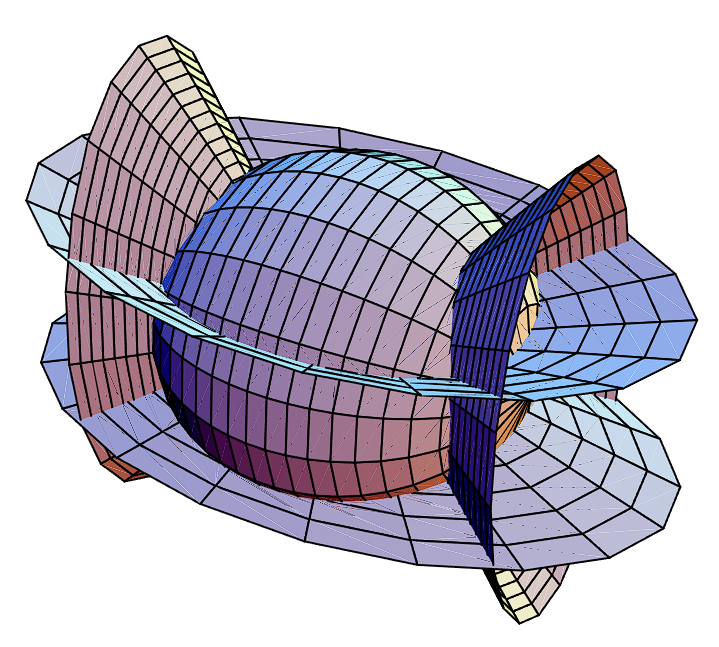
\includegraphics[width=\textwidth]{special_functions_fig/ellipsoidal_coordinates_schematic_diagram.png}
	\end{subfigure}
	\hfill
	\begin{subfigure}[b]{0.68\textwidth}
		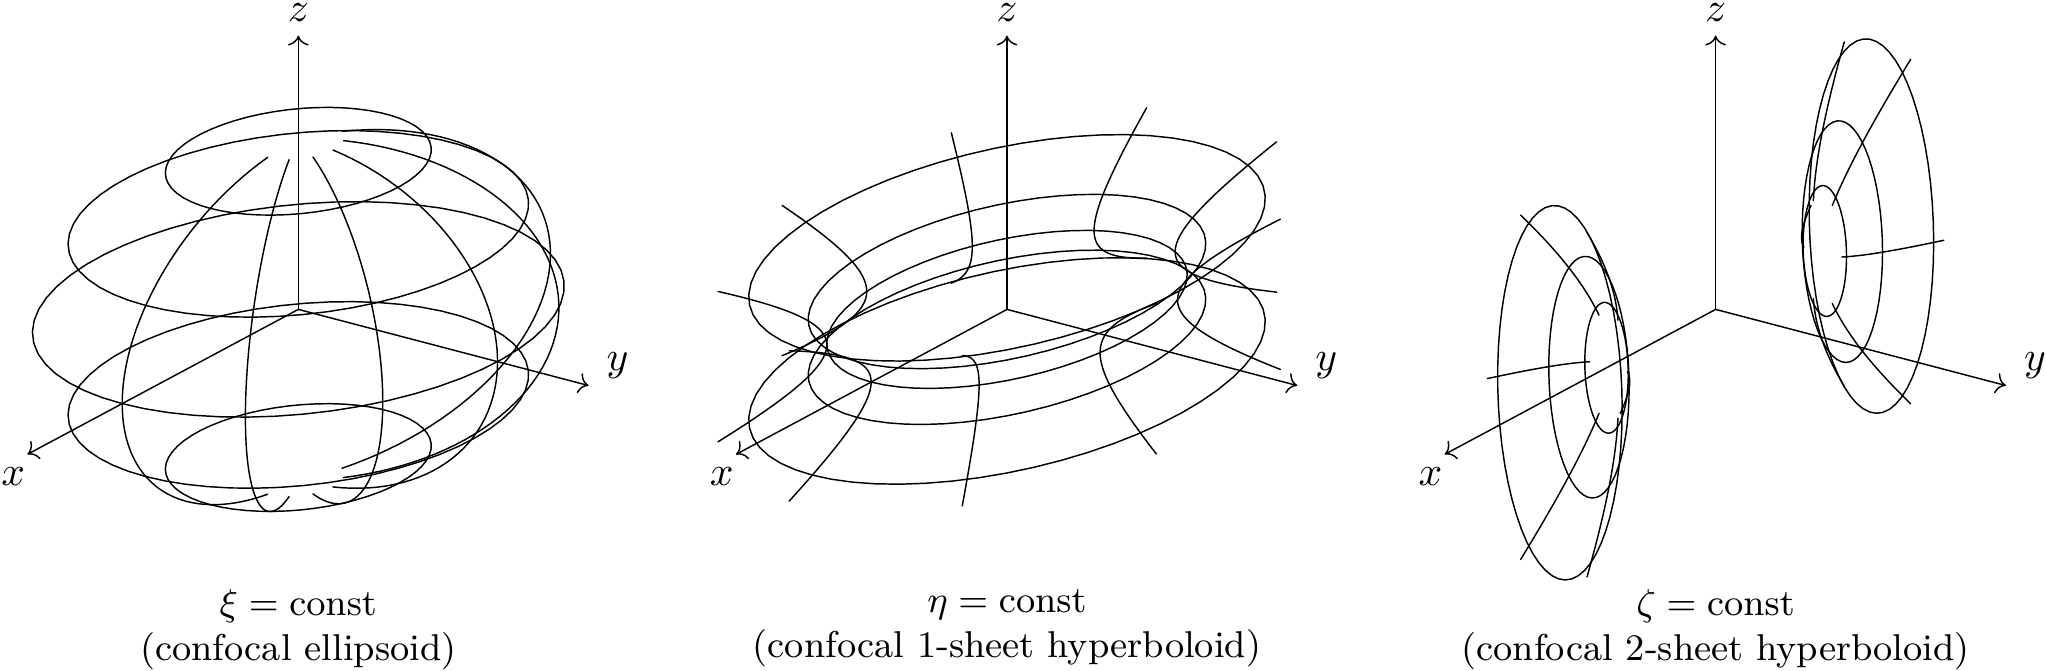
\includegraphics[width=\textwidth]{special_functions_fig/ellipsoidal_coordinates_schematic_diagram_2.png}
	\end{subfigure}
	\caption{椭球坐标示意图}
	\label{fig:ellipsoidal_coordinates}
\end{figure}

易知
\begin{align*}
	\frac{x^{2}}{a^{2}}+\frac{y^{2}}{b^{2}}+\frac{z^{2}}{c^{2}}
	 & =1+\frac{\xi\,\eta\,\zeta}{a^{2}b^{2}c^{2}},                                             \\
	a^{2}b^{2}c^{2}\Bigl(\frac{x^{2}}{a^{4}}+\frac{y^{2}}{b^{4}}+\frac{z^{2}}{c^{4}}\Bigr)
	 & =\xi\,\eta+\eta\,\zeta+\zeta\,\xi
	+\frac{\xi\,\eta\,\zeta\,(a^{2}b^{2}+b^{2}c^{2}+c^{2}a^{2})}{a^{2}b^{2}c^{2}},
\end{align*}
\(-c^{2}\le\xi<0\) 对应椭球\((a,b,c)\)的内部；\(\xi>0\) 对应椭球外部；\(\xi=0\) 对应椭球表面.

易证，椭球坐标系是正交系，其距离元为
\begin{align*}
	\dd s^{2}=\dd x^{2}+\dd y^{2}+\dd z^{2}
	=h_{\xi}^{2}\,\dd \xi^{2}+h_{\eta}^{2}\,\dd \eta^{2}+h_{\zeta}^{2}\,\dd \zeta^{2},
\end{align*}
其中
\begin{align*}
	 & h_{\xi}=\frac12\sqrt{\frac{(\xi-\eta)(\xi-\zeta)}{\varphi(\xi)}},\quad
	h_{\eta}=\frac12\sqrt{\frac{(\eta-\xi)(\eta-\zeta)}{\varphi(\eta)}},\quad
	h_{\zeta}=\frac12\sqrt{\frac{(\zeta-\xi)(\zeta-\eta)}{\varphi(\zeta)}}    \\
	 & \varphi(\Theta)=(a^{2}+\Theta)(b^{2}+\Theta)(c^{2}+\Theta).
\end{align*}

进而体积元为
\begin{align*}
	\dd V
	=h_{\xi}\,h_{\eta}\,h_{\zeta}\,\dd \xi\, \dd \eta\, \dd \zeta=-\frac{(\xi-\eta)(\eta-\zeta)(\zeta-\xi)}
	{8\sqrt{-\varphi(\xi)\,\varphi(\eta)\,\varphi(\zeta)}}\,
	\dd \xi\,\dd \eta\,\dd \zeta.
\end{align*}

拉普拉斯算子为
\begin{align*}
	\nabla^{2}
	=\frac{4\sqrt{\varphi(\xi)}}{(\xi-\eta)(\xi-\zeta)}
	\frac{\partial}{\partial\xi}\Bigl(\sqrt{\varphi(\xi)}\,
	\frac{\partial}{\partial\xi}\Bigr)\nonumber
	-\frac{4\sqrt{-\varphi(\eta)}}{(\eta-\xi)(\eta-\zeta)}
	\frac{\partial}{\partial\eta}\Bigl(\sqrt{-\varphi(\eta)}\,
	\frac{\partial}{\partial\eta}\Bigr)\nonumber
	+\frac{4\sqrt{\varphi(\zeta)}}{(\zeta-\xi)(\zeta-\eta)}
	\frac{\partial}{\partial\zeta}\Bigl(\sqrt{\varphi(\zeta)}\,
	\frac{\partial}{\partial\zeta}\Bigr).
\end{align*}

基矢为
\begin{align*}
	\uv{e}_{\xi}
	 & =\frac{1}{h_{\xi}}\frac{\partial\vb{r}}{\partial\xi}
	=\frac{1}{2h_{\xi}}\Bigl(\frac{x}{a^{2}+\xi}\uv{e}_{x}
	+\frac{y}{b^{2}+\xi}\uv{e}_{y}
	+\frac{z}{c^{2}+\xi}\uv{e}_{z}\Bigr),\notag                 \\
	\uv{e}_{\eta}
	 & =\frac{1}{h_{\eta}}\frac{\partial\vb{r}}{\partial\eta}
	=\frac{1}{2h_{\eta}}\Bigl(\frac{x}{a^{2}+\eta}\uv{e}_{x}
	+\frac{y}{b^{2}+\eta}\uv{e}_{y}
	+\frac{z}{c^{2}+\eta}\uv{e}_{z}\Bigr),\notag                \\
	\uv{e}_{\zeta}
	 & =\frac{1}{h_{\zeta}}\frac{\partial\vb{r}}{\partial\zeta}
	=\frac{1}{2h_{\zeta}}\Bigl(\frac{x}{a^{2}+\zeta}\uv{e}_{x}
	+\frac{y}{b^{2}+\zeta}\uv{e}_{y}
	+\frac{z}{c^{2}+\zeta}\uv{e}_{z}\Bigr).
\end{align*}

易知，\(\uv{e}_{\Theta}\;(\Theta=\xi/\,\eta/\,\zeta)\) 恰为等 \(\Theta\) 面
\begin{align*}
	\frac{x^{2}}{a^{2}+\Theta}+\frac{y^{2}}{b^{2}+\Theta}+\frac{z^{2}}{c^{2}+\Theta}=1
\end{align*}
的单位法向量，\(\uv{e}_{\xi}|_{\xi=0}\)恰为原椭球表面的外法向量.

若某函数恰可分离变量为形式
\(\Psi(\xi,\eta,\zeta)=f(\xi,\eta,\zeta)\,g(\xi)\)，则
\begin{align*}
	\nabla^{2}\Psi
	=g\,\nabla^{2}f
	+\frac{4\,f\,\sqrt{\varphi(\xi)}}{(\xi-\eta)(\xi-\zeta)}
	\Bigl[
		2\frac{\partial f}{\partial\xi}\frac{1}{f}\,
		\sqrt{\varphi(\xi)}\,\frac{\dd g}{\dd \xi}
		+\frac{\dd}{\dd \xi}\Bigl(\sqrt{\varphi(\xi)}\,\frac{\dd g}{\dd \xi}\Bigr)
		\Bigr].
\end{align*}